\newcommand{\SUM}{\raise1.5pt\hbox{$\scriptstyle\sum_{s=1}^N$}}
\newcommand {\cc}{\tiny(CC)}
\newcommand {\fc}{\tiny(FC)}
\newcommand {\dat}{\tiny(dat)}

\chapter{ICE} \label{Sec:ICE}


\section{Introduction}
The work presented here describes a multi-material CFD approach
designed to solve ``full physics" simulations of dynamic fluid
structure interactions involving large deformations and material
transformations (e.g., phase change).  ``Full physics" refers to
problems involving strong interactions between the fluid field and
solid field temperatures and velocities, with a full Navier Stokes
representation of fluid materials and the transient, nonlinear
response of solid materials.  These interactions may include chemical
or physical transformation between the solid and fluid fields.

The theoretical and algorithmic basis for the multi-material CFD
algorithm presented here is based on a body of work of several
investigators at Los Alamos National Laboratory, primarily Bryan
Kashiwa, Rick Rauenzahn and Matt Lewis.  Several reports by these
researchers are publicly available and are cited herein.  It is
largely through our personal interactions that we have been able to
bring these ideas to bear on the simulations described herein.


An exposition of the governing equations is given in the next section,
followed by an algorithmic description of the solution of those equations.
This description is first done separately for the materials in the Eulerian
and Lagrangian frames of reference, before details associated with the
integrated approach are given. 

\subsection{Governing Equations}\label{sec:governing_equations}
The governing multi-material model equations are stated and described, but
not developed, here.  Their development can be found in~\cite{kashiwa2000}.
Here, our intent is to identify the quantities of interest, of which there
are eight, as well as those equations (or closure models) which govern their
behavior.  Consider a collection of $N$ materials, and let the subscript r
signify one of the materials, such that $\rmr = 1, 2, 3, \dots, N$.  In an
arbitary volume of space $V(\bfx,t)$, the averaged thermodynamic state of a
material is given by the vector $[M_\rmr, \bfu_\rmr, e_\rmr, T_\rmr, v_\rmr,
\theta_\rmr, \sig_\rmr, p]$, the elements of which are the r-material mass,
velocity, internal energy, temperature, specific volume, volume fraction,
stress, and the equilibration pressure.  The r-material averaged density is
$\rho_\rmr = M_\rmr/V$.  The rate of change of the state in a volume moving
with the velocity of r-material is:
%
\noindent
%__________________________________
% mass
\begin{eqnarray}
{1\over V}{D_\rmr M_\rmr \over Dt} &=&
\SUM\Gamma_{\rmr\rms}
\label{eqmassr} \\
\nonumber \\
%__________________________________
% momentum
{1\over V}{D_\rmr (M_\rmr \bfu_\rmr) \over Dt} &=&
\theta_\rmr \bnabla\cdot\sig +
\bnabla\cdot\theta_\rmr(\sig_\rmr - \sig) + 
\rho_\rmr\bfg + 
\SUM \bff_{\rmr\rms} + 
\SUM \bfu_{\rmr\rms}^+ 
\Gamma_{\rmr\rms}
\label{eqmomr}\\ \nonumber \\
%__________________________________
% internal energy
{1\over V}{D_\rmr (M_\rmr e_\rmr) \over Dt} &=& -
\rho_\rmr p {D_\rmr v_\rmr\over Dt} +
\theta_\rmr\taubold_\rmr:\nabla\bfu_\rmr - 
\bnabla\cdot\bfj_\rmr +
\SUM q_{\rmr\rms} +
\SUM h_{\rmr\rms}^+ 
\Gamma_{\rmr\rms}
\label{eqenergyr}
\end{eqnarray}

Equations (\ref{eqmassr}-\ref{eqenergyr}) are the averaged model equations
for mass, momentum, and internal energy of r-material, in which $\sig$ is
the mean mixture stress, taken here to be isotropic, so that $\sig = -p\bfI$
in terms of the hydrodynamic pressure $p$.  The effects of turbulence have
been explicitly omitted from these equations, and the subsequent solution,
for the sake of simplicity.  However, including the effects of turbulence
is not precluded by either the model or the solution method used here.

In Eq. (\ref{eqmomr}) the term $\sum_{s=1}^{N}\bff_{\rmr\rms}$ signifies
a model for the momentum exchange among materials.  This term results from
the deviation of the r-field stress from the mean stress, averaged, and is
typically modeled as a function of the relative velocity between materials
at a point. (For a two material problem this term might look like $\bff_{12}
= K_{12}\theta_1\theta_2(\bfu_1 - \bfu_2)$ where the coefficient $K_{12}$
determines the rate at which momentum is transferred between materials).
Likewise, in Eq. (\ref{eqenergyr}), $\sum_{\rms=1}^{N} q_{\rmr\rms}$
represents an exchange of heat energy among materials.  For a two material
problem $q_{12} = H_{12}\theta_1\theta_2(T_2 - T_1)$ where $T_\rmr$ is the
r-material temperature and the coefficient $H_{\rmr\rms}$ is analogous to a
convective heat transfer rate coefficient.  The heat flux is $\bfj_\rmr =
-\rho_\rmr b_\rmr \bnabla T_\rmr$ where the thermal diffusion coefficient
$b_\rmr$ includes both molecular and turbulent effects (when the turbulence
is included).

In Eqs. (\ref{eqmassr}-\ref{eqenergyr}) the term $\Gamma_{\rmr\rms}$ is
the rate of mass conversion from s-material into r-material, for example,
the burning of a solid or liquid reactant into gaseous products.  The rate at which
mass conversion occurs is governed by a reaction model.  In Eqs. (\ref{eqmomr})
and (\ref{eqenergyr}), the velocity $\bfu_{\rmr\rms}^+$ and the enthalpy
$h_{\rmr\rms}^+$ are those of the s-material that is converted into r-material.
These are simply the mean values associated with the donor material.

The temperature $T_\rmr$, specific volume $v_\rmr$, volume fraction
$\theta_\rmr$, and hydrodynamic pressure $p$ are related to the r-material
mass density, $\rho_\rmr$, and specific internal energy, $e_\rmr$, by way
of equations of state.  The four relations for the four quantites $(T_\rmr,
v_\rmr, \theta_\rmr, p)$ are:

%
\begin{eqnarray}
e_\rmr &=& e_\rmr(v_\rmr, T_\rmr) \label{caloric} \\
v_\rmr &=& v_\rmr(p, T_\rmr) \label{thermal} \\
\theta_\rmr &=& \rho_\rmr v_\rmr \label{thedef} \\
0 &=& 1 - \SUM\rho_\rms v_\rms
\label{mmeos}
\end{eqnarray}
%
Equations (\ref{caloric}) and (\ref{thermal}) are, respectively, the caloric
and thermal equations of state.  Equation (\ref{thedef}) defines the volume
fraction, $\theta$, as the volume of r-material per total material volume,
and with that definition, Equation (\ref{mmeos}), referred to as the
multi-material equation of state, follows.  It defines the unique value of
the hydrodynamic pressure $p$ that allows arbitrary masses of the multiple
materials to identically fill the volume $V$.  This pressure is called the
``equilibration'' pressure \cite{kashiwaICE94}.

A closure relation is still needed for the material stress $\sig_\rmr$.
For a fluid $\sig_\rmr = -p\bfI + \taubold_\rmr$ where the deviatoric stress
is well known for Newtonian fluids.  For a solid, the material stress is the
Cauchy stress.  The Cauchy stress is computed using a solid constitutive
model and may depend on the the rate of deformation, the current state of
deformation ($\bfE$), the temperature, and possibly a number of history
variables.  Such a relationship may be expressed as:

%
\begin{equation}
{\sig}_\rmr \equiv \sig_\rmr(\bnabla\bfu_\rmr, \bfE_\rmr, T_\rmr,~ \dots)
\label{conslaw}
\end{equation}
%
The approach described here imposes no restrictions on the types of constitutive relations
that can be considered.  More specific discussion of some of the models
used in this work is found in Sec.~\ref{sec:models}

Equations (\ref{eqmassr}-\ref{conslaw}) form a set of eight equations for
the eight-element state vector, \\ $[M_\rmr, \bfu_\rmr, e_\rmr, T_\rmr,
v_\rmr, \theta_\rmr, \sig_\rmr, p]$, for any arbitrary volume of space $V$
moving with the r-material velocity.  The approach described here uses the
reference frame most suitable for a particular material type.  As such,
there is no guarantee that arbitrary volumes will remain coincident for
materials described in different reference frames.  This problem is addressed
by treating the specific volume as a dynamic variable of the material state
which is integrated forward in time from initial conditions.  In so doing,
at any time, the total volume associated with all of the materials is given by:
%
\begin{eqnarray}
V_t = {\raise1.5pt\hbox{$\scriptstyle\sum_{r=1}^N$}} M_\rmr v_\rmr
\end{eqnarray}
%
so the volume fraction is $\theta_\rmr = M_\rmr v_\rmr / V_t$ (which sums
to one by definition).  An evolution equation for the r-material specific
volume, derived from the time variation of Eqs. (\ref{caloric}-\ref{mmeos}),
has been developed in \cite{kashiwa2000}.  It is stated here as:
%
\begin{eqnarray}
{1\over V}{D_\rmr (M_\rmr v_\rmr) \over Dt} =
f_\rmr^{\theta} \bnabla \cdot \bfu &+&
\left[v_\rmr \Gamma_\rmr -
f_\rmr^{\theta} \SUM
v_\rms \Gamma_\rms \right]  \nonumber \\ &+&
\left[\theta_\rmr
\beta_\rmr {D_\rmr T_\rmr\over Dt} -
f_\rmr^{\theta} \SUM
\theta_\rms \beta_\rms {D_\rms T_\rms\over Dt} \right] \; .
\label{eqspvolr}
\end{eqnarray}

where $f_\rmr^{\theta} = {{\theta_\rmr \kappa_\rmr} \over
{\raise1pt\hbox{${\scriptstyle\sum_{\rms =1}^N}$}} \theta_\rms\kappa_\rms}$,
and $\kappa_\rmr$ is the r-material bulk compressibility.

The evaluation of the multi-material equation of state (Eq. (\ref{mmeos}))
is still required in order to determine an equilibrium pressure that results
in a common value for the  pressure, as well as specific volumes that fill
the total volume identically.

A description of the means by which numerical solutions to the equations in
Section~\ref{sec:ICE:algorithm} are found is presented next.  This begins
with separate, brief overviews of the methodologies used for the Eulerian
and Lagrangian reference frames.  The algorithmic details necesssary for
integrating them to achieve a tightly coupled fluid-structure interaction
capability is provided in Sec.~\ref{sec:MPMICE}.

\section{Algorithm Description}\label{sec:ICE:algorithm}

The Eulerian method implemented here is a cell-centered, finite volume,
multi-material version of the ICE (for Implicit, Continuous fluid, Eulerian)
method \cite{harlowamsden68} developed by Kashiwa and others at Los Alamos
National Laboratory \cite{kashiwaCCICE94}.  ``Cell-centered'' means that all
elements of the state are colocated at the grid cell-center (in contrast to
a staggered grid, in which velocity components may be centered at the faces
of grid cells, for example).  This colocation is particularly important
in regions where a material mass is vanishing.  By using the same control
volume for mass and momentum it can be assured that as the material mass goes
to zero, the mass and momentum also go to zero at the same rate, leaving a
well-defined velocity.  The technique is fully compressible, allowing wide
generality in the types of problems that can be addressed.
 
Our use of the cell-centered ICE method employs time splitting: first,
a Lagrangian step updates the state due to the physics of the conservation
laws (i.e., right hand side of Eqs.~{\ref{eqmassr}-\ref{eqenergyr}}); this
is followed by an Eulerian step, in which the change due to advection is
evaluated.  For solution in the Eulerian frame, the method is well developed
and described in \cite{kashiwaCCICE94}.

In the mixed frame approach used here, a modification to the multi-material
equation of state is needed.  Equation (\ref{mmeos}) is unambiguous when all
materials are fluids or in cases of a flow consisting of dispersed solid grains
in a carrier fluid.  However in fluid-structure problems the stress state of a
submerged structure may be strongly directional, and the isotropic part of the
stress has nothing to do with the hydrodynamic (equilibration) pressure $p$.
The equilibrium that typically exists between a fluid and a solid is at the
interface between the two materials: there the normal part of the traction
equals the pressure exerted by the fluid on the solid over the interface.
Because the orientation of the interface is not explicitly known at any
point (it is effectively lost in the averaging) such an equilibrium cannot
be computed.

The difficulty, and the modification that resolves it, can be understood by
considering a solid material in tension coexisting with a gas.  For solid
materials, the equation of state is the bulk part of the constitutive response
(that is, the isotropic part of the Cauchy stress versus specific volume and
temperature).  If one attempts to equate the isotropic part of the stress
with the fluid pressure, there exist regions in pressure-volume space for
which Eq. (\ref{mmeos}) has no physical solutions (because the gas pressure
is only positive).  This can be seen schematically in Fig.~\ref{vpfig}, which
sketches equations of state for a gas and a solid, at an arbitrary temperature.

Recall that the isothermal compressiblity is the negative slope of the
specific volume versus pressure.  Embedded structures considered here are
solids and, at low pressure, possess a much smaller compressibility than
the gasses in which they are submerged.  Nevertheless the variation of
condensed phase specific volume can be important at very high pressures,
where the compressibilities of the gas and condensed phase materials can
become comparable (as in a detonation wave, for example).  Because the speed of
shock waves in materials is determined by their equations of state, obtaining
accurate high pressure behavior is an important goal of our FSI studies.

To compensate for the lack of directional information for the embedded
surfaces, we evaluate the solid phase equations of state in two parts.
Above a specified postive threshold pressure (typically 1 atmosphere),
the full equation of state is respected; below that threshold pressure, the
solid phase pressure follows a polynomial chosen to be $C^1$ continuous at the
threshold value and which approaches zero as the specific volume becomes large.
The effect is to decouple the solid phase specific volume from the stress when
the isotropic part of the stress falls below a threshold value.  In regions
of coexistence at states below the threshold pressure, $p$ tends to behave
according to the fluid equation of state (due to the greater compressibility)
while in regions of pure condensed phase material $p$ tends rapidly toward
zero and the full material stress dominates the dynamics as it should.

%FIXME
%\subsection{Uintah Implementation}
%- to be filled in\\

\section{Uintah Specification}
%______________________________________________________________________
\subsection{Basic Inputs}
Each Uintah component is invoked using a single executable called
\it sus \normalfont, which chooses the type of simulation
to execute based on the \it SimulationComponent \normalfont tag in the
input file.  In the case of ICE simulations, this looks like:
%
\begin{Verbatim}[fontsize=\footnotesize]
 <SimulationComponent type="ice" />
\end{Verbatim}
%
near the top of the inputfile.  The system of units \bf{must }\normalfont be
consistent (mks, cgs) and the majority of input files will be in Meter-Kilogram-Sec
system.  For small length scale simulations, it is advantageous to use "bomb units", 
which are a consistent set of units for microgram mass scales, centimeter length scales
and micosecond timescales.  A conversion table of relevant physical quantities from mks
to bomb units can be found in Appendix \ref{appendixBombUnits}.

%FIXME
%\red{ discuss  first order and second order advection}

%\red{ discuss timestep scheme.  We mainly use aggressive}
%
%______________________________________________________________________
\subsection{Semi-Implicit Pressure Solve}
The equation for the change in the pressure field $\Delta{P}$ during a given
timestep is given by
%
\begin{equation}
    \label{eq:delP}
     \frac{dP}{dt} = 
     \frac{\sum \limits_{{m}=1}^N  \frac{\dot{m}} {V \rho^{o}_m} 
        -  \sum \limits_{{m}=1}^N \nabla \cdot \widehat{\theta_m} \vec{U_m}^{*^{f}}}
          {\sum \limits_{{m}=1}^N \frac{\theta_m}{\rho^{o}_m c_m^2} }
\end{equation}
%
which can be written in matrix form $Ax = b$ and solved with a linear solver.  Details on the
notation, discretization of Eq. \ref{eq:delP} and the formation of $A$
and $b$ can be found in
%
\begin{Verbatim}[fontsize=\footnotesize]
 src/CCA/Components/ICE/Docs/implicitPressSolve.pdf
\end{Verbatim}
%
The linear system $Ax = b$ can be solved using the default Uintah:conjugate
gradient solver (cg) (slow) or one of the many that are available
through the scalable linear solvers and preconditioner package hypre
\cite{ref:hypre}. Experience has shown that the most efficient hypre
preconditioner and solver are the pfmg and cg respectively.  Below are
typical values for both the Uintah:cg and hypre:cg solver
%
\begin{Verbatim}[fontsize=\footnotesize]
<ImplicitSolver>
   <max_outer_iterations>         20    </max_outer_iterations>
   <outer_iteration_tolerance>    1e-8  </outer_iteration_tolerance>
   <iters_before_timestep_restart> 5    </iters_before_timestep_restart>
   <Parameters variable="implicitPressure">

    <tolerance>     1.e-10  </tolerance>
    
    <!-- CGSolver options -->
    <norm>     LInfinity  </norm>
    <criteria> Absolute   </criteria>

    <!-- Hypre options -->
    <solver>         cg      </solver>
    <preconditioner> pfmg    </preconditioner>
    <maxiterations>  7500    </maxiterations>
    <npre>           1       </npre>
    <npost>          1       </npost>
    <skip>           0       </skip>
    <jump>           0       </jump>
   </Parameters>
</ImplicitSolver>
\end{Verbatim}
%
If the user is interested in altering the tolerance to which the equations are solved they should look at
\begin{Verbatim}[fontsize=\footnotesize]
<tolerance> and <outer_iteration_tolerance>
\end{Verbatim} 
%

\noindent
\footnotesize
\begin{tabular}{l p{8cm}}
XML tag &  Description\\
\hline
\hline
max\_outer\_iterations           &  maximum number of iterations in the outer loop of the pressure solve.\\
outer\_iteration\_tolerance      &  tolerance XXXXDX\\
iters\_before\_timestep\_restart &  \footnotesize number of outer iterations before a timestep is restarted\\
tolerance                        &   XXXX\\
\hline
\end{tabular}
\normalsize\\
\\
%______________________________________________________________________
\subsection{Physical Constants}
The gravitational constant and a reference pressure are specified in:
\begin{Verbatim}[fontsize=\footnotesize]
<PhysicalConstants>
   <gravity>            [0,0,0]   </gravity>
   <reference_pressure> 101325.0  </reference_pressure>
</PhysicalConstants>
\end{Verbatim}
%
%______________________________________________________________________
\subsection{Material Properties} \label{sec:ICEmat_props}
For each ICE material the thermodynamic and transport properties must be
specified, in addition to the initial conditions of the fluid inside of
each geom\_object.  Below is the an example of how to specify an invisid
ideal gas over square region with dimensions $6m X 6m X 6m$.  The initial
conditions of the gas in that region are $T=300, \rho=1.179, v_x=1,v_y=2,
v_z=3$ \big{(}Note, the pressure XML tag is not used as an initial condition
and is simply there to make the user aware of what the pressure would be at
that thermodynamic state.\big{)}
%
\begin{Verbatim}[fontsize=\footnotesize]
<MaterialProperties>
   <ICE>
     <material>
       <EOS type = "ideal_gas">                </EOS>
       <dynamic_viscosity>   0.0               </dynamic_viscosity>
       <thermal_conductivity>0.0               </thermal_conductivity>
       <specific_heat>      716.0              </specific_heat>
       <gamma>              1.4                </gamma>
       <geom_object>
           <box label="wholeDomain">
               <min>       [ 0.0, 0.0, 0.0 ]  </min>
               <max>       [ 6.0, 6.0, 6.0 ]  </max>
           </box>
           <res>                 [2,2,2]      </res>
           <velocity>      [1.,2.,3.]         </velocity>
           <density>       1.1792946927374306 </density>
           <pressure>      101325.0           </pressure>     
           <temperature>   300.0              </temperature>
       </geom_object>
     </material>
  </ICE>       
</MaterialProperties>
\end{Verbatim}
%______________________________________________________________________
\subsection{Equation of State}
Below is a list of the various equations of state, along with the user defined
constants, that are available.  The reader should consult the literature for
the theoretical development and applicability of the equations of state to
the problem being solved.
%
%
The most commonly used EOS is the ideal gas law
\begin{equation}
  p = (\gamma -1) c_v \rho T
\end{equation}
%
and is specified in the input file with:
%
\begin{Verbatim}[fontsize=\footnotesize]
<EOS type="ideal_gas"/>
\end{Verbatim}
%
The Thomsen Hartka EOS for cold liquid water (1-100 atm pressure range)
is specified with \cite{ref:Thomsen,ref:bejan}
%
\begin{Verbatim}[fontsize=\footnotesize]
<EOS type="Thomsen_Hartka_water">
  <a>  2.0e-7     </a>    <!-- (K/Pa)     -->    
  <b>  2.6        </b>    <!-- (J/kg K^2) -->
  <co> 4205.7     </co>   <!-- (J/Kg K)   -->
  <ko> 5.0e-10    </ko>   <!-- (1/Pa)     -->
  <To> 277.0      </To>   <!-- (K)        -->
  <L>  8.0e-6     </L>    <!-- (1/K^2)    -->
  <vo> 1.00008e-3 </vo>   <!-- (m^3/kg)   -->
</EOS>
\end{Verbatim}
% 
%
The input specification for the ``JWLC'', ``JWL++'' and ``Murnahan'' equations of state from \cite{ref:JWL} are: 
\begin{Verbatim}[fontsize=\footnotesize]
<EOS type = "JWLC">
  <A>   2.9867e11   </A>
  <B>   4.11706e9   </B>
  <C>   7.206147e8  </C>
  <R1>    4.95      </R1>
  <R2>    1.15      </R2>
  <om>    0.35      </om>
  <rho0>  1160.0    </rho0>
</EOS>
\end{Verbatim}
%
\begin{Verbatim}[fontsize=\footnotesize]
<EOS type = "JWL">
  <A>     1.6689e12 </A>
  <B>     5.969e10  </B>
  <R1>      5.9     </R1>
  <R2>      2.1     </R2>
  <om>      0.45    </om>
  <rho0>  1835.0    </rho0>
</EOS>
\end{Verbatim}
%
\begin{Verbatim}[fontsize=\footnotesize]
<EOS type = "Murnahan">
  <n>     7.4       </n>
  <K>     39.0e-11  </K>
  <rho0>  1160.0    </rho0>
  <P0>    101325.0  </P0>
</EOS>
\end{Verbatim}
%
The ``hard sphere'' or ``Abel'' equation of state for dense gases is
%
\begin{equation}
  p(v - b) = RT
\end{equation}
%
where b corresponds to the volume occupied by the molecules themselves \cite{ref:thompson}.
Input parameters are specified using:
%
\begin{Verbatim}[fontsize=\footnotesize]
<EOS type="hard_sphere_gas">
   <b> 1.4e-3 </b>
</EOS>
\end{Verbatim}
%
%
Non-idea gas equation of state used in HMX combustion simulations the Twu-Sim-Tassone(TST) EOS
is
\begin{equation}
  p = \frac{ (\gamma -1)c_v T }{ v - b} - \frac{ a }{(v+3.0b)(v-0.5b)}
\end{equation}
%
Input parameters are specified using:
%
\begin{Verbatim}[fontsize=\footnotesize]
<EOS type="TST">
  <a>       -260.1385968     </a>
  <b>       7.955153678e-4   </b>
  <u>       -0.5             </u>
  <w>       3.0              </w>
  <Gamma>   1.63             </Gamma>
</EOS>
\end{Verbatim}
%
%
The input parameters for the Tillotson equation of state \cite{ref:gathers} for soils :
%
\begin{Verbatim}[fontsize=\footnotesize]
<EOS type = "Tillotson">
  <a>       .5      </a>
  <b>       1.3     </b>
  <A>       4.5e9   </A>
  <B>       3.0e9   </B>
  <E0>      6.e6    </E0>
  <Es>      3.2e6   </Es>
  <Esp>     18.0e6  </Esp>
  <alpha>   5.0     </alpha>
  <beta>    5.0     </beta>
  <rho0>    1700.0  </rho0>
</EOS>
\end{Verbatim}
%
%______________________________________________________________________
\subsection{Exchange Properties}
The heat and momentum exchange coefficients $K_{rs}$ and $H_{rs}$, which
determine the rate at which momentum and heat are transferred between
materials, and are specified in the following format.
%
\begin{Verbatim}[fontsize=\footnotesize]
0->1,   0->2,  0->3
        1->2,  1->3
               2->3
\end{Verbatim}
%
For a two material problem the coefficients would be:
%
\begin{Verbatim}[fontsize=\footnotesize]
<exchange_properties> 
   <exchange_coefficients>
      <momentum>  [0, 1e15, 1e15 ]     </momentum>
      <heat>      [0, 1e10, 1e10 ]     </heat>  
   </exchange_coefficients>
</exchange_properties>
\end{Verbatim}
%
%
%______________________________________________________________________
\subsection{BoundaryConditions}
Boundary conditions must be specified on each face of the computational
domain $(x^-, x^+, y^-, y^+,z^-,z^+)$ for the variables $P, \bf{u},
T, \rho, v$ for each material.  The three main types of numerical
boundary conditions that can be applied are ``Neumann",  ``Dirichlet" and
``Symmetric".  A Neumann boundary condition is used to set the gradient
or $\frac{\partial{q}}{\partial{n}}|_{surface} = value$ at the boundary.
The value of the primative variable in the boundary cell is given by,

%
\begin{equation}
    q[\text{boundary cell}] = q[\text{interior cell}] - value * dn;
\end{equation}
%
if we use a first order upwind discretization of the gradient.  Dirichlet
boundary conditions set the value of primative variable in the boundary
cell using
%
\begin{equation}
    q[\text{boundary cell}] =  value;
\end{equation}
%
\begin{Verbatim}[fontsize=\footnotesize]
<Grid>
  <BoundaryConditions>
    <Face side = "x-">
      <BCType id = "0"   label = "Pressure"     var = "Neumann">
                            <value> 0. </value>
      </BCType>
      <BCType id = "all" label = "Velocity"     var = "Neumann">
                            <value> [0.,0.,0.] </value>
      </BCType>
      <BCType id = "all" label = "Temperature"  var = "Neumann">
                            <value> 0.0 </value>
      </BCType>
      <BCType id = "all" label = "Density"      var = "Neumann">
                            <value> 0.0 </value>
      </BCType>
      <BCType id = "all" label = "SpecificVol"  var = "computeFromDensity">
                            <value> 0.0  </value>
      </BCType>
    </Face>
      .
      [other faces]
      .
  </BoundaryConditions>
</Grid>
\end{Verbatim}
There is also the field tag \TT{id = "all".}  In principal, one could set
different boundary condition types for different materials.  In practice,
this is rarely used, so the usage illustrated here should be used.  Note that
pressure field id is always 0.  Symmetric boundary conditions are set using:
%
\begin{Verbatim}[fontsize=\footnotesize]
<Face side = "y-">
    <BCType id = "all" label = "Symmetric" var = "symmetry"> </BCType>
</Face>
\end{Verbatim}
%
In addition to ``Dirichlet'', ``Neumann'', and ``Symmetric'' type boundary
conditions ICE has several custom or experimental  boundary conditions the user can
access.  The ``Sine'' boundary condition was designed to impose a pulsating
pressure wave in the boundary cells by applying
%
\begin{equation} \label{eq:pSine}
  p = p_{reference} + A  sin(\omega t)
\end{equation}
%
The input file parameters that control the frequency and magnitude of the  wave are: 
\begin{Verbatim}[fontsize=\footnotesize]
<SINE_BC>
  <omega>    1000 </omega>
  <A>        800 </A>
</SINE_BC>
\end{Verbatim}
and to specify them add
\begin{Verbatim}[fontsize=\footnotesize]
<BCType id = "0"   label = "Pressure"     var = "Sine"> 
                      <value> 0.0 </value> 
</BCType> 
<BCType id = "0"   label = "Temperature"  var = "Sine"> 
                      <value> 0.0 </value>
</BCType>
\end{Verbatim}
%
to the input file.
%
For non-reflective boundary conditions the user should specify the ``LODI''
or locally one-dimensional invisid type \cite{ref:Sutherland}

\begin{Verbatim}[fontsize=\footnotesize]
<LODI>
  <press_infinity> 1.0132500000010138e+05  </press_infinity>
  <sigma>          0.27                    </sigma>
  <ice_material_index> 0                   </ice_material_index>
</LODI>
\end{Verbatim}
%
and
%
\begin{Verbatim}[fontsize=\footnotesize]
<Face side = "x+">
  <BCType id = "0"   label = "Pressure"     var = "LODI">
                        <value> 0. </value>                
  </BCType>
  <BCType id = "0"   label = "Velocity"     var = "LODI">
                        <value> [0.,0.,0.] </value>
  </BCType>
  <BCType id = "0"   label = "Temperature"  var = "LODI">
                        <value> 0.0 </value>
  </BCType>
  <BCType id = "0"   label = "Density"      var = "LODI">
                        <value> 0.0 </value>
  </BCType>
  <BCType id = '0' label = "SpecificVol" var = "computeFromDensity">
                        <value> 0.0 </value>
  </BCType>
</Face> 
\end{Verbatim}
%
This boundary condition is designed to suppress all the unwanted effects of an
artifical boundary. \bf This BC is computationally expensive, not entirely
effective and should be used with caution\normalfont.  In flow fields where
there are no passing through the outlet of the domain it reduces
the reflected pressure waves significantly.
%FIXME
%Table below shows some of the

\subsection{Output Variable Names}
There are numerous variables that can be saved during a simulation.  The table below is
a list of the most commonly saved variables.  To see the entire list ICE
specfic variables available to the user run
%
\begin{Verbatim}[fontsize=\footnotesize]
  inputs/labelNames ice
\end{Verbatim}
% 
Dimensions are given in mass (M), length (L), time (t) and tempertare
(T).  Bold face label names signify vectors quantities.  The location of
the variable on the grid is denoted by (CC) for the cell-centered or (FC)
for face-centered.  Conserved quantities that are summed over all cells, every
timestep, and written to a ``dat" file inside of the \TT{uda} directory are denoted with (dat).
%
%__________________________________
\newpage
\begin {center}
\scriptsize
\begin{tabular}{lllp{8cm}}
\label{table:iceLabels}
\\
LabelName & & Description\\
\hline
\hline
delP\_Dilatate        &$M/Lt^2$    & change in pressure during the, \cc.\\ 
delP\_MassX           &$M/Lt^2$    & change in pressure due to mass addition, \cc. \\

eng\_adv              & $ML^2/t^2$ & energy of a material after the advection task, \cc.\\
eng\_exch\_error      & $ML^2/t^2$ & $\sum_{i=1}^{\text{AllCells}} \text{Internal Energy After Exchange Process} - $ \\
                      &            & $\sum_{i=1}^{\text{AllCells}}\text{Internal Energy Before Exchange Process}$, \dat.\\
eng\_L\_ME\_CC        & $ML^2/t^2$ & Energy of a material after the exchange task and just before the advection task, \cc.\\

%heatCond\_src\_CC
imp\_delP             & $M/Lt^2$ & \cc.\\
%int\_eng\_L\_CC
%intE\_source\_CC
KineticEnergy         & $ML^2/t^2$ &   $\sum_{i=1}^{\text{AllCells}} (0.5 m \vec(v)^2)_i$, \dat.\\

mach                  & & Mach number, \cc.\\
mag\_div\_vel\_CC     & & Magnitude of the divergence of the velocity, \cc.\\
mag\_grad\_press\_CC  & & Magnitude of the gradient of the pressure, \cc.\\
mag\_grad\_rho\_CC    & & Magnitude of the gradient of the density, \cc.\\
mag\_grad\_temp\_CC   & & Magnitude of the gradient of the temperature, \cc.\\
mag\_grad\_vol\_frac\_CC
                      & & Magnitude of the gradient of the volume fraction, \cc.\\
mass\_adv             & $M$ & Mass of a material after the advection task, \cc.\\
mass\_L\_CC           & $M$ & Mass of a material just before the advection task, \cc.\\

%matrix
%max\_RHS
modelEng\_src         & $ML^2/t^2$ & Energy source term, computed from a reaction model, \cc.\\
modelMass\_src        & $M$        & Mass source term, computed from a reaction model, \cc.\\
\bf{modelMom\_src}    & $ML/t$     & Momentum source term, computed from a reaction model, \cc.\\
modelVol\_src         & & Volume source term,  computed from a reaction model, \cc.\\

%mom\_adv
\bf{mom\_exch\_error} & $ML/t$ &  $\sum_{i=1}^{\text{AllCells}} \text{Momemtum After Exchange Process} - $ \\
                      &        &  $\sum_{i=1}^{\text{AllCells}} \text{Momentum Before Exchange Process}$, \dat.\\
\bf{mom\_L\_CC}       & $ML/t$ & Momemtum before momentum exchange task, \cc.\\
\bf{mom\_L\_ME\_CC}   & $ML/t$ & Momentum after momentum exchange task, \cc.\\
\bf{mom\_source\_CC}  & $ML/t$ & All sources of momentum,\cc.\\

press\_CC             & $M/Lt^2$ & Pressure  $P = P_{\text{equilibration}} + \Delta{P}$, \cc.\\
press\_equil\_CC      & $M/Lt^2$ & Pressure after the compute equilibration task, \cc.\\
pressX\_FC            & $M/Lt^2$ & Pressure on the $x^{-,+}$ cell faces, \fc.\\
pressY\_FC            & $M/Lt^2$ & Pressure on the $y^{-,+}$ cell faces, \fc.\\
pressZ\_FC            & $M/Lt^2$ & Pressure on the $z^{-,+}$ cell faces, \fc.\\

rho\_CC               & $M/L^3$  & Density  of each material, \cc.\\
%rhs

specific\_heat        & $L^2/t^2T$ & Constant Specific Heat, \cc.\\
speedSound\_CC        & $L/t$      & Speed of sound  of each material, \cc.\\
sp\_vol\_adv          & & \\
sp\_vol\_CC           & $L3/M$     & Specific volume of each material, \cc.\\
%sp\_vol\_L\_CC
%sp\_vol\_src\_CC
%sp\_volX\_FC
%sp\_volY\_FC
%sp\_volZ\_FC
%sum\_imp\_delP

temp\_CC              & $T$  & Temperature  of each material, \cc.\\
TempX\_FC             & $T$  & temperature on the $x^{-,+}$ cell faces, \fc.\\
TempY\_FC             & $T$  & temperature on the $y^{-,+}$ cell faces, \fc.\\
TempZ\_FC             & $T$  & temperature on the $z^{-,+}$ cell faces, \fc.\\
thermalCond           & $ML/t^3T$ & Thermal conductivity, \cc.\\

TotalIntEng           & $ML^2/t^2$ & $\sum_{i=1}^{\text{AllCells}} (m c_v T)_i$, \dat.\\
TotalMass             & $M$        & $\sum_{i=1}^{\text{AllCells}} m_i$, \dat.\\
TotalMomentum         & $ML/t$     & $\sum_{i=1}^{\text{AllCells}} (m \vec{v})_i$, \dat.\\
%turb\_viscosity\_CC

uvel\_FC              & $L/t$  & x-component of velocity, before momentum exchange, \fc.\\
uvel\_FCME            & $L/t$  & x-component of velocity, after momentum exchange task, \fc.\\

\bf{vel\_CC}          & $L/t$  & Velocity at the end of a timestep, \cc.\\ 
viscosity             & $M/Lt$ & Dynamic viscosity, \cc.\\
vol\_frac\_CC         &        & Volume fraction of each material, \cc.\\
vol\_fracX\_FC        &        & Volume fraction on the $x^{-,+}$ cell faces, \fc.\\
vol\_fracY\_FC        &        & Volume fraction on the $y^{-,+}$ cell faces, \fc.\\
vol\_fracZ\_FC        &        & Volume fraction on the $z^{-,+}$ cell faces, \fc.\\
vvel\_FC              & $L/t$ & y-component of velocity, before momentum exchange task, \fc.\\
vvel\_FCME            & $L/t$ & y-component of velocity, after momentum exchange task, \fc.\\
wvel\_FC              & $L/t$ & z-component of velocity, before momentum exchange, \fc.\\
wvel\_FCME            & $L/t$ & z-component of velocity, after momentum exchange task, \fc.\\

\hline
\end{tabular}
\normalfont
\end{center}
\normalsize
%______________________________________________________________________
The variables,
\TT{mag\_div\_vel\_CC,
mag\_grad\_press\_CC,  
mag\_grad\_rho\_CC, 
mag\_grad\_temp\_CC,   
mag\_grad\_vol\_frac\_CC,}
are the magnitude of the gradient or divergence of the respective primative variable.  
If the user visual To  are large and based on this information
the adaptive mesh cell refinement criteria can be set.

%______________________________________________________________________
%  XML tags
\newpage
Below is a list of the \TT{XML} tags pertaining specifically to \TT{ICE} problems.

\subsection{XML tag description}
%__________________________________
\begin {center}
\scriptsize
\begin{tabular}{lllp{8cm}}
XML tag & Type & Dimensions & Description\\
\hline
\hline
cfl                   & double &               &    Courant Number.\\
gravity               & Vector & $[L/t^2]$     &    gravitational acceleration, $\vec{g}$.\\
\\
\underline{\footnotesize{global material properties}} & & &\\
dynamic\_viscosity    & double & $[M/Lt]$      &    viscosity, $\mu$.\\
thermal\_conditucivity& double & $[ML/t^3T]$   &    thermal conductivity, $k$\\
specific\_heat        & double & $[L^2/t^2 T]$ &   $c_p$\\
gamma                 & double &               &    ratio of specific heats, $\gamma$.\\
\\
\underline{\footnotesize{geometry object related}} & & &\\
res                   & vector &               &    resolution used for defining geometry objects.\\
velocity              & vector & $[L/t]$       &    initial velocity, $\vec{u}$.\\
density               & double & $[M/L^3]$     &    initial density, $\rho$.\\
temperature           & double & $[T]$         &    initial temperature, $T$.\\
pressure              & double &               &    Not used. \\
\\
\underline{\footnotesize{AMR Parameters}} & & & \\
orderOfInterpolation  & integer &              &    Order of interpolation at the coarse/fine interfaces. \\
do\_Refluxing         & boolean &              &    on/off switch for correcting the flux of mass, momentum, and energy at the
                                                    course/fine interfaces.\\
\hline
\end{tabular}
\end{center}


%______________________________________________________________________
\newpage
\section{Examples}
Below are several example problems that illustrate the wide range of problems
that can be solved using the ICE algorithm.  Where possible simulation
results are compared to exact solutions or high fidelity numerical results.
Note in order to run the post processing scripts the user should have a
recent version of Octave installed.  To visualize the results the visualization
package VisIT should be used.  VisIT session files are included.
 
\subsection*{\center Poiseuille Flow}
\addcontentsline{toc}{subsection}{Poiseuille Flow}
\subsubsection*{\underline{Problem Description}}
The Poiseuille flow problem is classical viscous flow problem in which flow is
driven through two parallel plates from fixed pressure gradient.  The pressure
gradient is balanced by the diffusion $x$ momentum in the $y$ direction.

\subsubsection*{\underline{Simulation Specifics}}
\begin{description} 
\footnotesize
\item [Component used:] \hfill ICE
\item [Input file name:] \hfill \TT{CouettePoiseuille.ups}\\
Edit this file and set the boundary condition for the velocity on the y+ = 0.0.
Change:
\begin{Verbatim}[fontsize=\footnotesize]
<BCType id = "0"   label = "Velocity"     var = "Dirichlet">
                       <value> [1.25,0.,0.] </value>
[to]
<BCType id = "0"   label = "Velocity"     var = "Dirichlet">
                      <value> [0,0.,0.] </value>
\end{Verbatim}
 
\item [Command used to run input file:]\hfill \\
\TT{mpirun -np 1 sus -solver hypre inputs/UintahRelease/ICE/CouettePoiseuille.ups}
\item [Postprocessing command:]\hfill \\
\TT{inputs/UintahRelease/ICE/compare\_Couette\-Poiseuille.m -uda Couette-Poiseuille.uda}\\
You must edit \TT{compare\_Couette\-Poiseuille.m} and set \TT{wallVel = 0}.
This will generate a postscript file Couette\-Poiseuille.ps

\item [Simulation Domain:]\hfill    1 x .01 x .01 m
\item [Cell Spacing:]\hfill \\ 
10 x 5 x 10 mm (Level 0)

\item [Example Runtimes:] \hfill \\
 8ish minutes   (1 processor, 2.66 GHz Xeon)

\item [Physical time simulated:] \hfill 15 sec.
\end{description}

\subsubsection*{\underline{Results}}
Figure \ref{fig:Poiseuille} shows a comparison of the exact and simulated u
velocity at time $t = 15sec$, 5 cells from the end of the domain.  The lower
plot shows the difference of the velocity $\|u - u_{exact}\|$.
%
\begin{figure}
  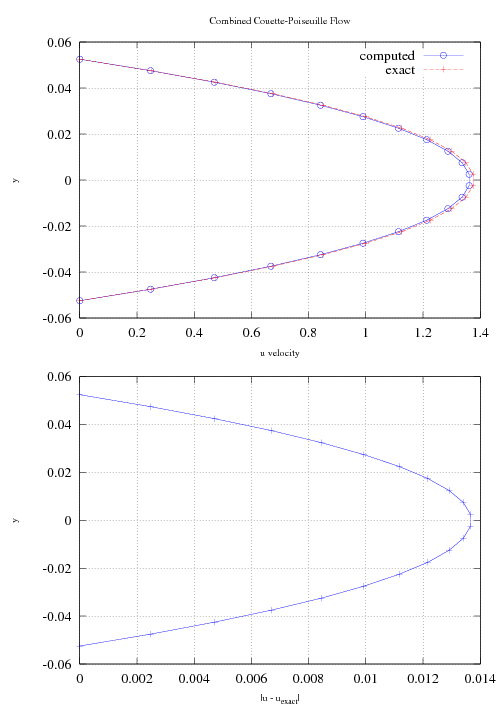
\includegraphics[scale=.80]{Poiseuille.png}
  \caption{ Comparison of $u$ velocity $t = 15sec$}
  \label{fig:Poiseuille}
  \end{figure}
\newpage
%
%______________________________________________________________________
\subsection*{\center Combined Couette-Poiseuille Flow}
\addcontentsline{toc}{subsection}{Combined Couette-Poiseuille Flow}
\subsubsection*{\underline{Problem Description}}
The combined Couette-Poiseuille flow problem is another classical viscous
flow problem in which flow is driven through a channel by a pressure gradient
and a wall moving.  The reduced x momentum equation differential is

\begin{equation}
  \mu \frac{d^2 u}{dy^2} = \frac{dp}{dx} = \text{constant}
\end{equation}
subject to the no slip boundary condition $u(\pm h) = \text{wall velocity}$,
where $h$ is half the height of the channel \cite{ref:white}.

\subsubsection*{\underline{Simulation Specifics}}
\begin{description} 
\footnotesize
\item [Component used:] \hfill ICE
\item [Input file name:] \hfill \TT{CouettePoiseuille.ups}
\item [Command used to run input file:]\hfill \\
\TT{mpirun -np 1 sus -solver hypre inputs/UintahRelease/ICE/CouettePoiseuille.ups}
\item [Postprocessing command:]\hfill \\
\TT{inputs/UintahRelease/ICE/compare\_Couette\-Poiseuille.m -uda Couette-Poiseuille.uda}\\
This Octave script will generate a postscript file Couette\-Poiseuille.ps

\item [Simulation Domain:]\hfill    1 x .01 x .01 m
\item [Cell Spacing:]\hfill \\ 
10 x 5 x 10 mm (Level 0)

\item [Example Runtimes:] \hfill \\
 8ish minutes   (1 processor, 2.66 GHz Xeon)

\item [Physical time simulated:] \hfill 15 sec.
\end{description}

\subsubsection*{\underline{Results}}
Figure \ref{fig:CombinedPoiseuille} shows a comparison of the exact and simulated u
velocity at time $t = 15sec$, 5 cells from the end of the domain.  The lower
plot shows the difference of the velocity $\|u - u_{exact}\|$.
%
\begin{figure}
  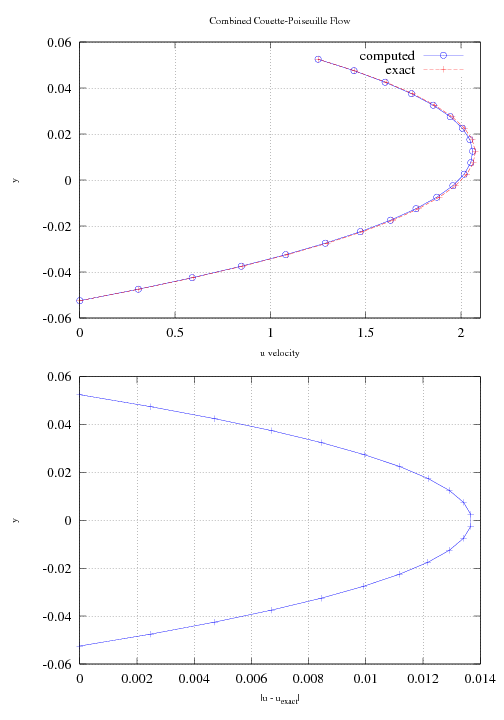
\includegraphics[scale=.85]{Couette-Poiseuille.png}
  \vspace{-20pt}
  \caption{ Comparison of $u$ velocity $t = 15sec$}
  \label{fig:CombinedPoiseuille}
  \end{figure}
\newpage
%
%______________________________________________________________________
\subsection*{\center Shock Tube}
\addcontentsline{toc}{subsection}{Shock Tube}
\subsubsection*{\underline{Problem Description}}
The shock tube problem is a standard 1D compressible flow problem that
has been used by many as a validation test case \cite{ref:laney, ref:sod, ref:toro}.
At time $t=0$ the computational domain is divided into two separate regions of
space by a diaphram, with each region at a different density and pressure.
The separated regions are at rest with a uniform temperature $=300K$.
The initial pressure ratio is $\frac{P_R}{P_L}  = 10$ and density ratio
is $\frac{\rho_R}{\rho_L} = 0.1$  The diaphram is instantly removed and a
traveling shockwave, discontinutity and expansion fan form.  The expansion
fan moves towards the left while the shockwave and contact discontinutity
move to the right.  This problem tests the algorithm's ability to capture
steep gradients and solve Eulers equations.
%
\subsubsection*{\underline{Simulation Specifics}}
\begin{description} 
\footnotesize
\item [Component used:] \hfill ICE
\item [Input file name:] \hfill \TT{rieman\_sm.ups}
\item [Command used to run input file:]\hfill \TT{sus inputs/UintahRelease/ICE/shockTube.ups}
\item [Postprocessing command:]\hfill \\
\TT{scripts/ICE/plot\_shockTube\_1L shockTube.uda y}\\
This Octave script will generate a postscript file shockTube.ps

\item [Simulation Domain:]\hfill    1 x .001 x .001 m
\item [Cell Spacing:]\hfill \\ 
1 x 1 x 1 mm (Level 0)

\item [Example Runtimes:] \hfill \\
 1 minute   (1 processor, 2.66 GHz Xeon)

\item [Physical time simulated:] \hfill 0.005 sec.
\end{description}

\subsubsection*{\underline{Results}}
Figure \ref{results.ST} shows a comparison of the exact versus simulated
results at time $t = 5msec$.
%
\begin{figure}
  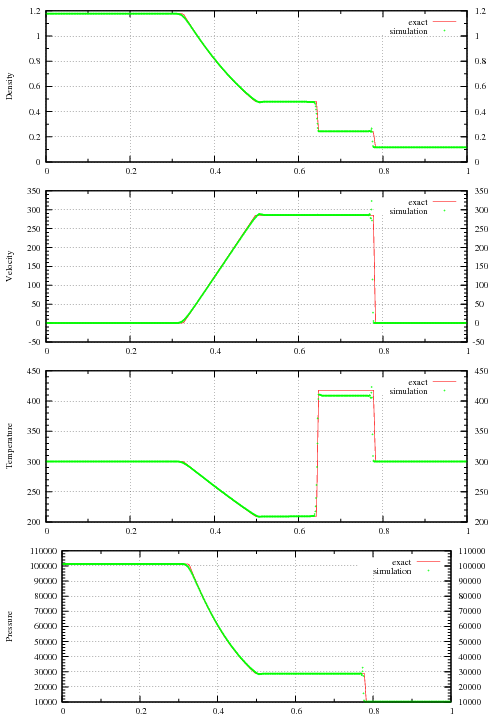
\includegraphics[scale=.65]{shockTube.png}
  \caption{Shock tube results at time $t = 5msec$}
  \label{results.ST}
  \end{figure}
\newpage
%
%__________________________________SHOCKTUBE AMR
\subsection*{\center Shock Tube with Adaptive Mesh Refinement}
\addcontentsline{toc}{subsection}{Shock Tube with Adaptive Mesh Refinement}
\subsubsection*{\underline{Simulation Specifics}}
\begin{description} 
\footnotesize
\item [Component used:] \hfill ICE
\item [Input file name:] \hfill \TT{shockTube\_AMR.ups}
\item [Command used to run input file:]\hfill\\ \TT{sus
inputs/UintahRelease/ICE/shockTube\_AMR.ups}
\item [Postprocessing command:]\hfill \\
\TT{../../src/scripts/ICE/plot\_shockTube\_AMR shockTube\_AMR.uda y}\\
This Octave script will generate a postscript file shockTube\_AMR.ps

\item [Simulation Domain:]\hfill    1 x .001 x .001 m
\item [Cell Spacing:] \hfill\\
10 x 1 x 1 mm (Level 0)\\
2.5 x 1 x1 mm (Level 1)\\
0.625 x1 x1 mm (Level 2)

\item [Example Runtimes:] \hfill \\
 2ish minutes   (1 processor, 2.66 GHz Xeon)

\item [Physical time simulated:] \hfill 0.0005 sec.

\end{description}

\subsubsection*{\underline{Results}}
Figure \ref{results.ST.AMR} shows a comparison of the exact versus simulated results at time $t = 5msec$.
\begin{figure}
  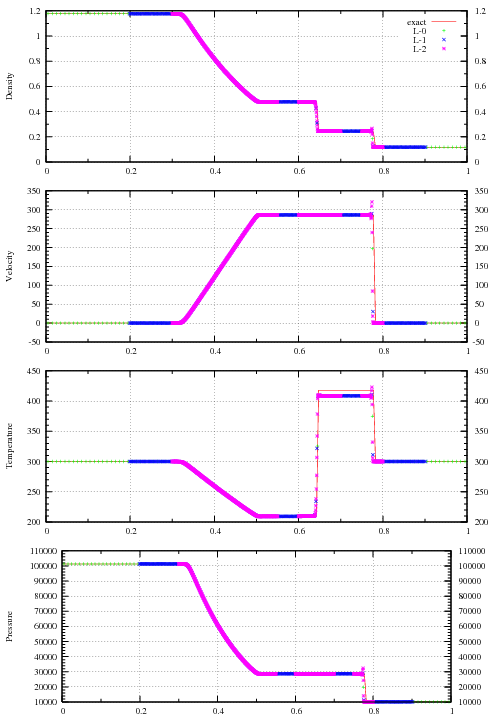
\includegraphics[scale=.85]{shockTube_AMR.png}
  \vspace{-10pt}
  \caption{Shock tube results at time $t = 5msec$}
  \label{results.ST.AMR}
  \end{figure}
\newpage
%
%__________________________________riemann2D
\subsection*{\center 2D Riemann Problem with Adaptive Mesh Refinement}
\addcontentsline{toc}{subsection}{2D Riemann Problem with Adaptive Mesh Refinement}
\subsubsection*{\underline{Problem Description}}
In two-dimensional Riemann problems there 15 different solutions that combine
rarefaction waves, shock waves and a slip line or contact discontinuities
\cite{ref:schulz_collins_glaz, ref:Liska_Wendroff}.  Here we simulate 4 slip
lines that form a symmetrical single vortex turning counter clockwise. At
time $t=0$ the computational domain is divided into four quadrants by the
lines $x = 1/2, y=1/2$  The initial condition for $V=(p, \rho, u, v)$ in the
four quadrants are $V_{ll}=(1, 1, -0.75, 0.5), V_{lr}=(1, 3, -0.75,-0.5),
V_{ul}=(1,2,0.75,0.5), V_{ur}=(1,1,0.75,-0.5)$ where, $p$ is pressure,
$\rho$ is the density of the polytropic gas, $u$ and $v$ are the $x$ and $y$
component of velocity.
\subsubsection*{\underline{Simulation Specifics}}
\begin{description} 
\footnotesize
\item [Component used:] \hfill ICE
\item [Input file name:] \hfill \TT{riemann2D\_AMR.ups}
\item [Command used to run input file:]\hfill \\
\TT{mpirun -np 5 sus inputs/UintahRelease/ICE/riemann2D\_AMR.ups}
\item [VisIT session file:]\hfill \TT{inputs/UintahRelease/ICE/riemann2D.session}
\item [Simulation Domain:]\hfill    0.96 x 0.96m x 0.1 m
\item [Cell Spacing:]\hfill \\ 
40  x 40  x 1 mm (Level 0)\\
10  x 10  x 1 mm (Level 1)\\
2.5 x 2.5 x 1 mm (Level 2)

\item [Example Runtimes:] \hfill \\
 5ish minutes   (5 processors, 2.66 GHz Xeon)
\item [Physical time simulated:] \hfill 0.3 sec.
\end{description}

\subsubsection*{\underline{Results}}
Figure \ref{fig:riemann2D} shows a flood and line contour plot(s) of the density of the gas at 0.03sec.
\begin{figure}
  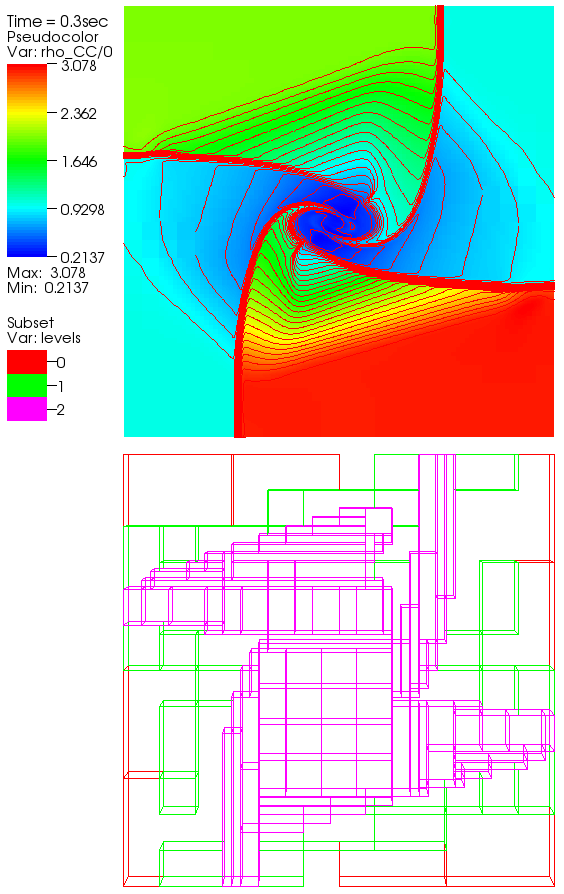
\includegraphics[scale=.6]{riemann2D.png}
  \caption{Contour plot of density for the 2D Riemann problem at time $t = 0.3sec$.  Bottom plot shows the outline of the patches on the 3 levels.}
  \label{fig:riemann2D}
  \end{figure}
\newpage
%
%__________________________________
\subsection*{\center Explosion 2D}
\addcontentsline{toc}{subsection}{Explosion 2D}
\subsubsection*{\underline{Problem Description}}
For the multidimensional blast wave orexplosion test is a standard compressible
flow problem that has been used by many as a validation test case.  At time
$t=0$ there is a circular region of gas at the center of the domain at a
relatively high pressure and density.  The expansion of high pressure gas
forms a circular shock wave and contact surface that expands into surrounding
atmosphere.  At the same time a circular rarefaction travels towards the
origin.  As the shock wave and contact surface move outwards they become
weaker and at some point the contact reverses direction and travels inward.
The rarefraction reflects from the center and forms an overexpanded region,
creating a shock that travels inward \cite{ref:toro}.  At time $t=0$ the
computational domain is divided into two region, circular high pressure region
with a radius $R=0.4$ and the surrounding box 2x2x0.1.  The initial condition
inside of the circular region were $(p=1, \rho=1, u=0, v=0)$  and outside
$(p=0.1, \rho=0.125, u=0, v=0).$  The fluid was an ideal, inviscid, polytropic gas.
%
\subsubsection*{\underline{Simulation Specifics}}
\begin{description} 
\item [Component used:] \hfill ICE
\item [Input file name:] \hfill \TT{explosion.ups}
\item [Command used to run input file:]\hfill \\
      \TT{mpirun -np 4 sus inputs/UintahRelease/ICE/explosion.ups}
\item [Visualization net file:]\hfill \TT{inputs/UintahRelease/ICE/Explosion.session}\\
\item [Postprocessing command:]\hfill \\
\tt scripts/ICE/plot\_explosion\_AMR Explosion\_AMR.uda y \normalfont \\
This Octave script will generate a postscript file explosion\_AMR.ps


\item [Simulation Domain:]\hfill    2 x 2 x .1
\item [Cell Spacing:]\hfill \\ 
62.5    x 62.5    x 10 (Level 0)\\
15.625  x 15.625  x 10 (Level 1)\\
3.9     x 3.9     x 10 (Level 2)

\item [Example Runtimes:] \hfill \\
 20 minutes   (4 processor, 2.66 GHz Xeon)

\item [Physical time simulated:] \hfill 0.25 (non-dimensional).

\end{description}

\subsubsection*{\underline{Results}}
Figures \ref{fig:pressExplode} and \ref{fig:rhoExplode} shows surface plots of the pressure and density at $t=0.25.$  
%\newpage
\begin{figure}
 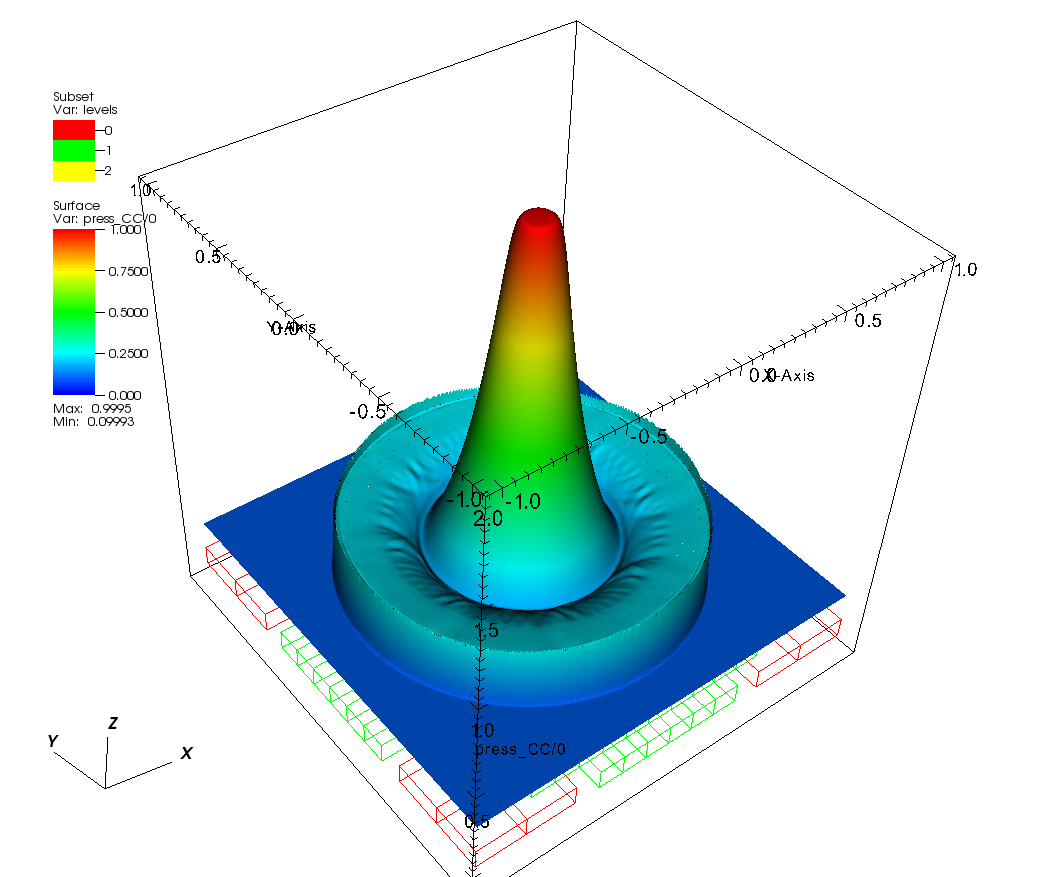
\includegraphics[scale=.5]{explode_press.png}
\caption{Pressure field at $t=0.25$}
\label{fig:pressExplode}
\end{figure}
%
%\newpage
\begin{figure}
  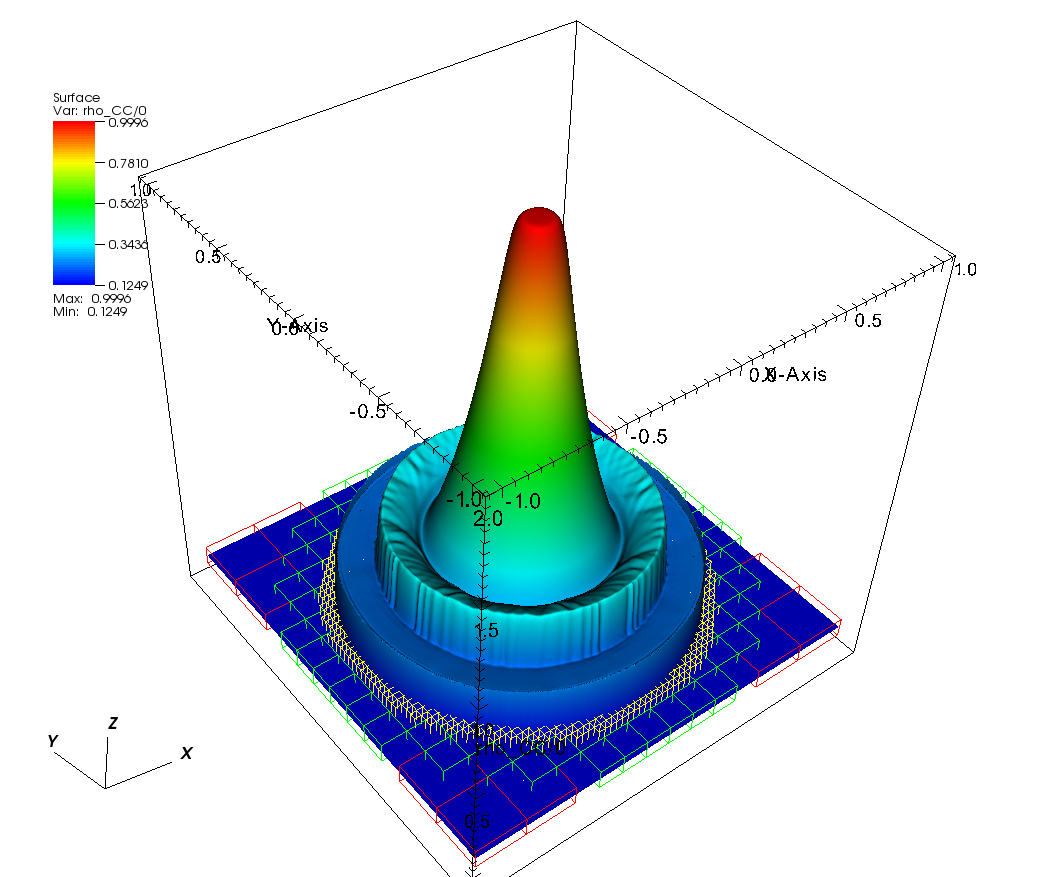
\includegraphics[scale=.5]{explode_rho.png}
  \caption{Density field at time $t=0.25$}
  \label{fig:rhoExplode}
\end{figure}
%\newpage
%
Since this test is symetrical we can use results from the equivalent 1 dimensional problem to compare against
%
\begin{figure}
  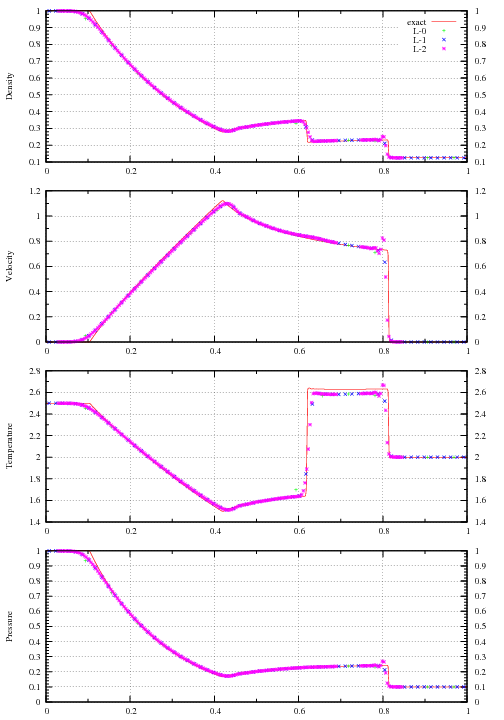
\includegraphics[scale=.75]{explode_1D.png}
  \caption{$t=0.25$}
  \label{fig:1dExplode}
\end{figure}
\newpage

%__________________________________
\subsection*{\center ANFO Rate Stick}
\addcontentsline{toc}{subsection}{ANFO Rate Stick}
\subsubsection*{\underline{Problem Description}}
A cylindrical stick ($r = 8 mm$) of Ammonium Nitrate Fuel Oil (ANFO) given an initial
velocity of $90 m/s$.  As it strikes the domain boundary, pressure is generated
sufficient to reach the initial pressure required to activate the 
JWL++~\cite{ref:JWL} detonation model.  This empirically based model results
in a steady state detonation that traverses the stick, consuming the solid 
explosive and generating high pressure gas.  The experimentally observed
curvature is generated at the detonation front, a feature that will not develop
in programmed burn models.  By running this simulation at
a variety of cylinder radii, one can observe the ''size effect", namely that
cylinders of larger radii will reach a higher steady state detonation velocity,
due to the increased effective confinement.  An infinite radius case can be
simulated by shrinking the computational domain to one cell in each of the
transverse directions.

%
\subsubsection*{\underline{Simulation Specifics}}
\begin{description}
\item [Component used:] \hfill ICE
\item [Input file name:] \hfill \TT{JWLpp8mmRS.ups}
\item [Command used to run input file:]\hfill \\
      \TT{mpirun -np 4 sus inputs/UintahRelease/ICE/JWLpp8mmRS.ups}
\item [Visualization net file:]\hfill \TT{inputs/UintahRelease/ICE/RateStick.session}\\

\item [Simulation Domain:]\hfill    0.1 m x 0.015 m x 0.015 m
\item [Cell Spacing:]\hfill \\
0.0005  x 0.0005  x 0.0005 (Level 0)\\

\item [Example Runtimes:] \hfill \\
 1.5 hours   (4 processor, 3.16 GHz Xeon)

\item [Physical time simulated:] \hfill 20.0 $\mu$seconds

\end{description}

\subsubsection*{\underline{Results}}
Figure \ref{fig:RateStick} shows a volume rendering of the density of the
reactant.  Note the curvature of the reaction zone.
\begin{figure}
 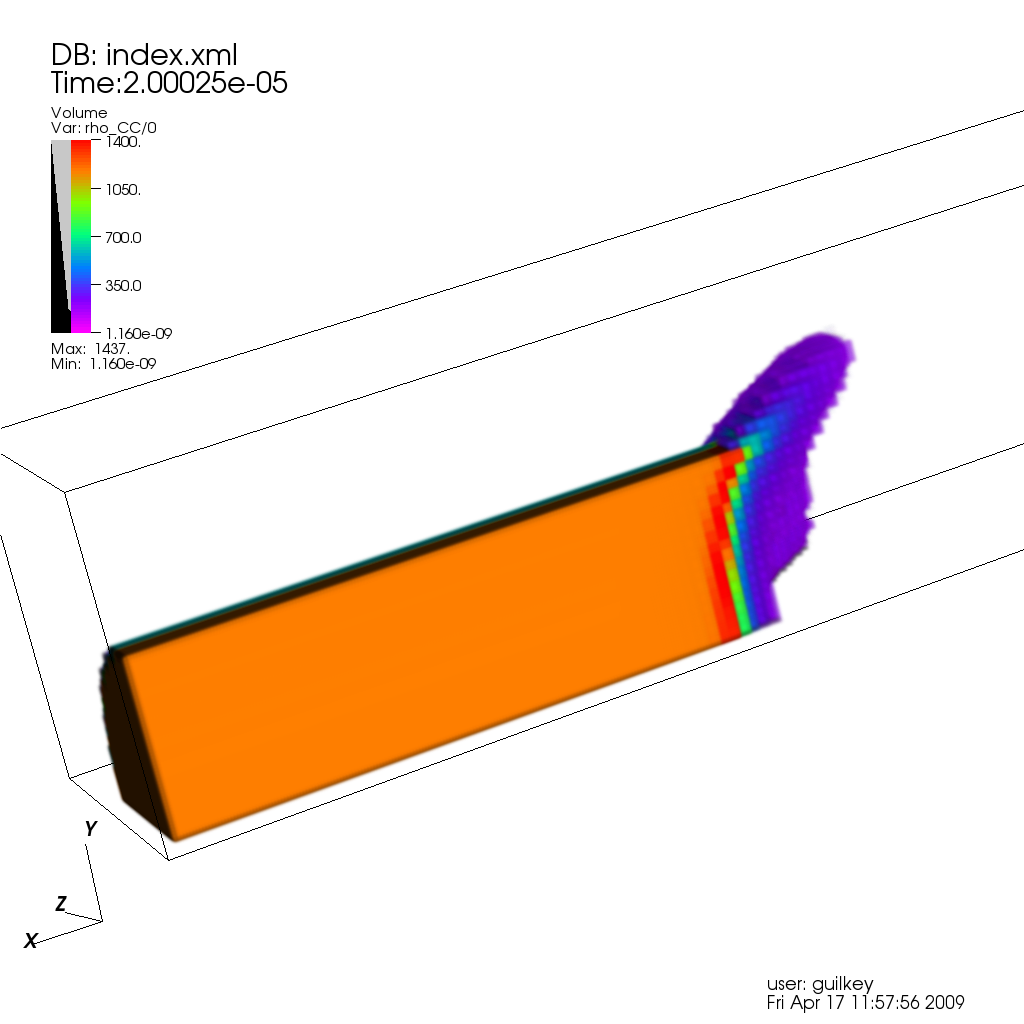
\includegraphics[scale=.5]{RateStick.png}
\caption{Density of reactant material.}
\label{fig:RateStick}
\end{figure}

\newpage

%__________________________________CH4 fire

%\section*{\center Methane Flame}
%\subsection*{\underline{Problem Description}}
%At $t=0$ Methane gas begin flowing from a $1m$ hole in the floor of the
%computational domain at a velocity of $1m/s$.  The methane mixes with the
%surrounding air, ignites and forms a puffing fire.  The main assumptions in
%this simulation are a) that the chemical reactions are taking place infinitely
%fast (equilibrium chemistry model) and b) that there is no radiative heat
%loss from the product gases.
%\subsection*{\underline{Simulation Specifics}}
%\begin{description} 
%\item [Component used:] \hfill ICE
%\item [Input file name:] \hfill CH4\_fire.ups
%\item [Command used to run input file:]\hfill sus CH4\_fire.ups \\
%Note you must have a link to the {\tt inputs} directory in the save directory as sus.  A table needed
%by the combustion model is inside the {\tt inputs} directory.
%\item [SCIRun visualization net file:]\hfill 3DFire\_Vol.srn \\
%
%
%\item [Simulation Domain:]\hfill    5 x 5 x 5 m
%\item [Cell Spacing:]\hfill \\ 
%3.3 x 3.3 x 3.3 cm (Level 0)
%
%
%\item [Example Runtimes:] \hfill \\
% 8 hours   (64 processor, 2.66 GHz Xeon)
%
%\item [Physical time simulated:] \hfill 3.4sec.
%
%\end{description}
%
%\section*{\underline{Results}}
%Figure \ref{results.CH4} shows a 3D view of the initial puff just before it leaves the computational
%doman.  
%\begin{figure}
%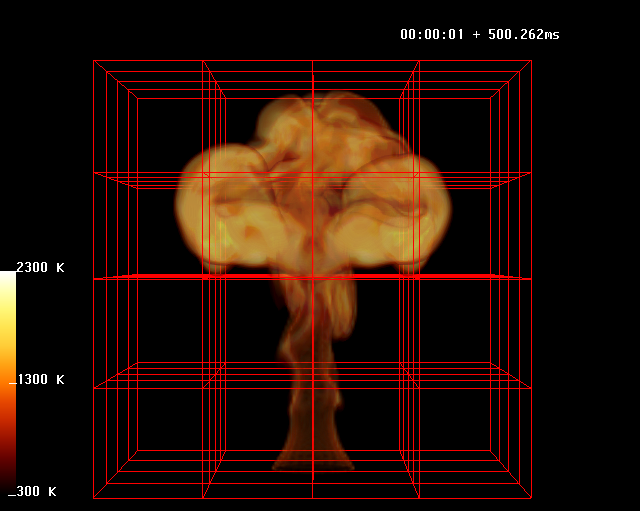
\includegraphics[scale=.66]{3DFire.png}
%\caption{Temperature field at time $t = 1.5 sec$}
%\label{results.CH4}
%\end{figure}
%\newpage

%\section{References}
\bibliographystyle{plain}
\bibliography{ice}


